\section{Statistical distributions and the tail-resolution problem}

This section establishes the probabilistic setting of the numerical experiments. We first formulate the practical problem that motivates binning, then introduce the three distributions used throughout the notes, and subsequently place them in the general language of probability measures, densities, cumulative distributions, and survival functions. The central result is that the visual and numerical difficulty of binning is controlled not only by sample size but also by the rate at which probability mass moves into the tail. Exponential, lognormal, and Pareto samples therefore provide a useful progression from light-tailed to genuinely scale-free behavior.

\subsection{The problem and the distributions to be analyzed}

Consider a positive sample $x_1,\ldots,x_n$ whose values may extend over a broad dynamic range. If the interval from the sample minimum to the sample maximum is divided into $K$ intervals of equal width, then each interval receives the same geometric length but generally not the same probability mass. This distinction is minor for a relatively compact distribution and decisive for a heavy-tailed one. In a Pareto sample, a small number of extreme observations can enlarge the total range by orders of magnitude, making the equal-width partition extremely coarse near the lower cutoff and nearly empty over much of the remaining range.

The experiments in these notes use $N=10^6$ observations from three continuous distributions. The exponential sample has scale $50$, the lognormal sample has logarithmic mean $\ln 150$ and logarithmic standard deviation $0.55$, and the Pareto sample has lower cutoff $x_{\min}=100$ and probability-density exponent $\alpha=2.5$. These numerical scales are chosen to place the synthetic observations on readable income-like ranges; they do not assert that an empirical income distribution follows any one of the three laws over its entire support.

The motivation from income data is concrete. The Brazilian analysis of Moura Jr. and Ribeiro \cite{MouraRibeiro2009} separates the dominant body of the distribution from a much smaller Pareto upper tail. A uniform discretization of the entire income range can therefore spend many bins on intervals containing very few households while under-resolving the body of the distribution. This is precisely the situation in which quantile bins or geometrically expanding bins can be more informative than a single equal-width partition.

Newman's review provides a second motivation through Zipf's law, the rank--size form of power-law behavior \cite{Newman2005}. Zipf originally studied rank--frequency regularities in language and related social data \cite{Zipf1949}, while the same mathematical structure later became standard in the analysis of city sizes and other broad distributions. If a positive random variable has Pareto CCDF $\overline F(x)\propto x^{-(\alpha-1)}$, then the expected rank $r$ of an observation of size $x$ in a sample of size $n$ satisfies, to leading order,
\begin{equation}
 r\simeq n\,\overline F(x)\propto x^{-(\alpha-1)},
\end{equation}
and therefore
\begin{equation}
 x(r)\propto r^{-1/(\alpha-1)}.
\end{equation}
The classical Zipf case $x(r)\propto r^{-1}$ corresponds to a Pareto density exponent near $\alpha=2$. This equivalence between a distributional tail and a rank--size law is important for the present problem because both representations become sensitive to sparse extreme observations, although they organize the information differently. Newman's treatment makes this connection explicit and also shows why logarithmic binning and cumulative representations are useful when the empirical tail spans several orders of magnitude \cite{Newman2005}.

\begin{figure}[!t]
\centering
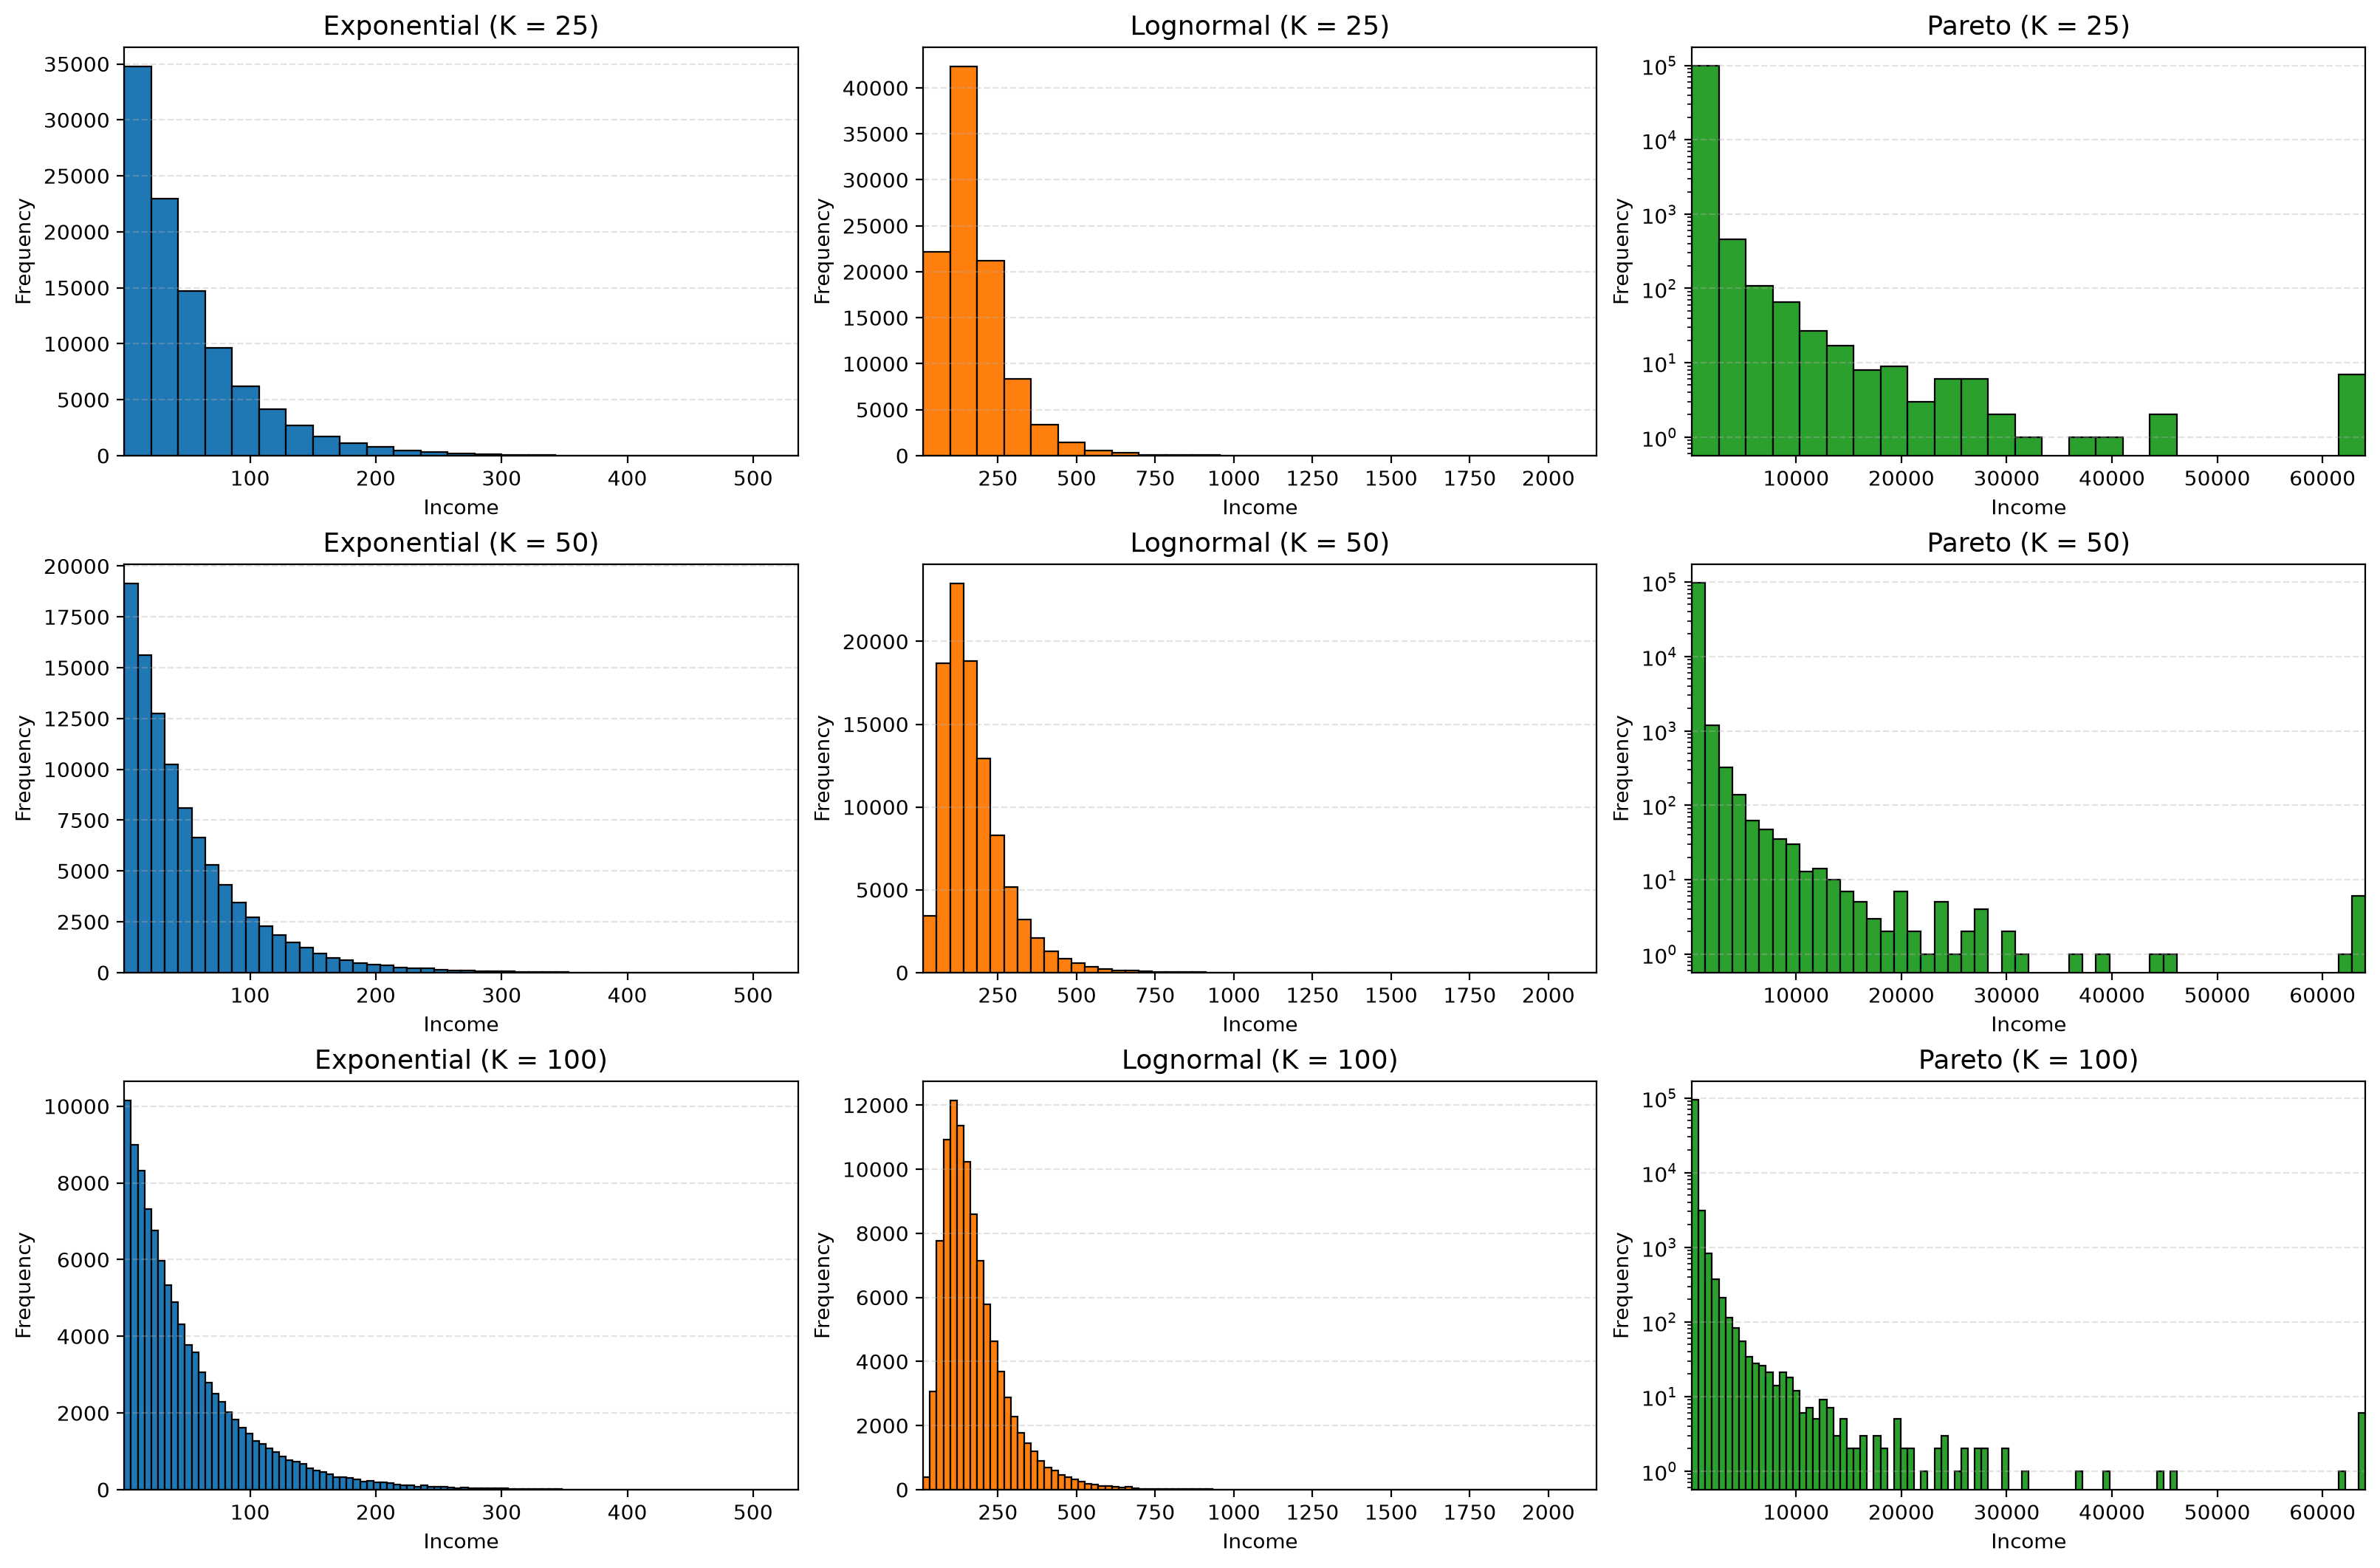
\includegraphics[width=0.92\textwidth]{histograms.png}
\caption{Synthetic exponential, lognormal, and Pareto samples represented with ordinary equal-width histograms for $K=25$, $50$, and $100$ bins. The Pareto panels retain a logarithmic vertical scale and a conservative visual truncation of only the most extreme observations. The same distributional parameters and random seed are used throughout the numerical comparison.}
\label{fig:synthetic-histograms}
\end{figure}

Figure~\ref{fig:synthetic-histograms} already displays the essential difficulty. The exponential and lognormal samples have ranges that remain manageable under ordinary binning. The Pareto sample, by contrast, develops a long sparse tail whose statistical structure is difficult to display with a fixed linear horizontal scale.

\subsection{Exponential, lognormal, and Pareto distributions}

The three laws used here differ fundamentally in their asymptotic decay. The exponential law possesses a characteristic scale and suppresses very large events exponentially. The lognormal law is broader and arises naturally from multiplicative mechanisms. The Pareto law has no exponential cutoff and assigns substantially more probability to extreme values. Standard probability references such as Ross \cite{Ross2014} provide the basic theory; the lognormal distribution and its empirical ubiquity are reviewed in detail by Limpert, Stahel, and Abbt \cite{LimpertStahelAbbt2001}.

\begin{definition}[Exponential distribution]
A nonnegative random variable $X$ is exponentially distributed with rate $\lambda>0$, written $X\sim\mathrm{Exp}(\lambda)$, if its probability density is
\begin{equation}
 f_X(x)=
 \begin{cases}
 \lambda e^{-\lambda x}, & x\geq 0,\\
 0, & x<0.
 \end{cases}
\end{equation}
Its cumulative and complementary cumulative distribution functions are
\begin{align}
 F_X(x) &= 1-e^{-\lambda x},\\
 \overline F_X(x) &= e^{-\lambda x},
\end{align}
for $x\geq 0$, and its first two moments are
\begin{equation}
 \mathbb{E}[X]=\frac{1}{\lambda},
 \qquad
 \mathrm{Var}(X)=\frac{1}{\lambda^2}.
\end{equation}
\end{definition}

The exponential law is the canonical waiting-time distribution of a homogeneous Poisson process. If events occur independently at constant rate $\lambda$, then the time between consecutive events is exponentially distributed. This makes the law a natural light-tailed benchmark: the probability of an observation larger than $x$ is suppressed as $e^{-\lambda x}$. In the binning experiments, this rapid decay gives a reference case in which the maximum grows slowly enough that ordinary equal-width intervals remain reasonably informative.

A broader distribution is obtained when randomness acts multiplicatively rather than additively. Taking logarithms converts products into sums, so repeated independent multiplicative factors naturally motivate a Gaussian approximation in log space. This leads to the next model.

\begin{definition}[Lognormal distribution]
A positive random variable $X$ is lognormally distributed with parameters $\mu\in\R$ and $\sigma>0$, written $X\sim\mathrm{Lognormal}(\mu,\sigma^2)$, if $Y=\ln X$ is normally distributed with mean $\mu$ and variance $\sigma^2$. Its density is
\begin{equation}
 f_X(x)=\frac{1}{x\sigma\sqrt{2\pi}}
 \exp\left[-\frac{(\ln x-\mu)^2}{2\sigma^2}\right],
 \qquad x>0.
\end{equation}
Its mean and variance are
\begin{align}
 \mathbb{E}[X] &= \exp\left(\mu+\frac{\sigma^2}{2}\right),\\
 \mathrm{Var}(X) &= \left(e^{\sigma^2}-1\right)e^{2\mu+\sigma^2}.
\end{align}
\end{definition}

The lognormal distribution is associated with multiplicative random mechanisms: products of many independent positive random factors become sums after taking logarithms, so a central-limit argument can produce approximate normality in log space. Newman \cite{Newman2005} explicitly discusses the lognormal law as an important broad-tailed alternative that can mimic power-law behavior over a finite range. This observation is methodologically important because apparent linearity over a short log--log interval does not uniquely identify a Pareto tail. Its moments are finite for every finite order, but its right tail is substantially broader than an exponential tail, which makes it a useful intermediate case between light-tailed and genuinely scale-free behavior.

The Pareto family changes the asymptotic regime qualitatively. Instead of exponential or lognormal suppression, probability decreases algebraically, so extreme observations remain much more frequent and the existence of moments depends directly on the tail exponent.

\begin{definition}[Pareto or continuous power-law distribution]
Let $x_{\min}>0$ and $\alpha>1$. A positive random variable $X$ follows the continuous power-law distribution used in these notes if
\begin{equation}
 f_X(x)=
 \begin{cases}
 (\alpha-1)x_{\min}^{\alpha-1}x^{-\alpha}, & x\geq x_{\min},\\
 0, & x<x_{\min}.
 \end{cases}
\label{eq:pareto-pdf}
\end{equation}
The corresponding complementary cumulative distribution is
\begin{equation}
 \overline F_X(x)=\mathbb{P}(X>x)
 =\left(\frac{x}{x_{\min}}\right)^{-(\alpha-1)},
 \qquad x\geq x_{\min}.
\label{eq:pareto-ccdf}
\end{equation}
\end{definition}

This notation follows Newman \cite{Newman2005}: $\alpha$ denotes the exponent of the probability density. In the common Pareto Type-I parameterization the shape parameter is instead $k=\alpha-1$. The distinction matters because the CCDF exponent is one unit smaller than the PDF exponent. Pareto's original work on income concentration provides the historical origin of this family \cite{Pareto1896}. The algebraic tail also implies that moment existence cannot be assumed automatically; it must be checked from the exponent.

\begin{proposition}[Existence of Pareto moments]
For the density in Eq.~\eqref{eq:pareto-pdf}, the moment $\mathbb{E}[X^m]$ is finite if and only if $\alpha>m+1$.
\end{proposition}

\begin{demonstration}
For $m\geq0$,
\begin{align}
\mathbb{E}[X^m]
&=(\alpha-1)x_{\min}^{\alpha-1}
\int_{x_{\min}}^{\infty}x^{m-\alpha}\,\dd x.
\end{align}
The improper integral converges precisely when $m-\alpha<-1$, equivalently when $\alpha>m+1$. Therefore the mean requires $\alpha>2$, while the variance requires $\alpha>3$.
\end{demonstration}

For the synthetic value $\alpha=2.5$, the theoretical mean exists but the variance diverges. Large observations are therefore not incidental anomalies; they are intrinsic to the model and strongly influence finite-sample summaries. This is one reason why a heavy-tail visualization should not be designed by simply suppressing the observations that make the plot inconvenient.

\subsection{Statistical distributions, PDF, CDF, and CCDF}

The preceding examples can be placed in a common measure-theoretic framework. The basic object is not a formula for a density but the probability law induced by a random variable. Densities, cumulative probabilities, and survival probabilities are alternative representations of that same law when the necessary regularity conditions hold.

\begin{definition}[Distribution of a random variable]
Let $(\Omega,\mathcal{F},\mathbb{P})$ be a probability space and let $X:\Omega\rightarrow\R$ be a measurable random variable. The distribution of $X$ is the probability measure $\mathbb{P}_X$ on the Borel sets of $\R$ defined by
\begin{equation}
 \mathbb{P}_X(A)=\mathbb{P}(X\in A),
 \qquad A\in\mathcal{B}(\R).
\end{equation}
\end{definition}

The distribution therefore assigns probability to measurable subsets of the state space. For continuous models it is often convenient to express this measure through a density, but the density itself should not be confused with a probability: it has units inverse to those of $X$, and probabilities are obtained only after integration over an interval.

\begin{definition}[Probability density function]
If $\mathbb{P}_X$ is absolutely continuous with respect to Lebesgue measure, then there exists a nonnegative function $f_X$ such that
\begin{equation}
 \mathbb{P}(a<X\leq b)=\int_a^b f_X(t)\,\dd t,
\end{equation}
with
\begin{equation}
 \int_{-\infty}^{\infty} f_X(t)\,\dd t=1.
\end{equation}
The function $f_X$ is the probability density function, or PDF.
\end{definition}

The density is local: it describes how rapidly probability accumulates per unit change in the variable. Cumulative representations instead collect probability from one side of the real line and are therefore naturally monotone. This distinction becomes useful in heavy-tail analysis because cumulative objects do not require a preliminary choice of bins.

\begin{definition}[Cumulative distribution function]
The cumulative distribution function of $X$ is
\begin{equation}
 F_X(x)=\mathbb{P}(X\leq x).
\end{equation}
For an absolutely continuous distribution,
\begin{equation}
 F_X(x)=\int_{-\infty}^{x}f_X(t)\,\dd t.
\end{equation}
\end{definition}

The CDF measures the probability accumulated to the left of $x$. In tail problems the complementary quantity is often more transparent because it directly reports the probability of exceeding a threshold and can be read as a survival probability.

\begin{definition}[Complementary cumulative distribution function]
The complementary cumulative distribution function, also called the survival function, is
\begin{equation}
 \overline F_X(x)=1-F_X(x)=\mathbb{P}(X>x).
\label{eq:ccdf-general}
\end{equation}
For continuous $X$, replacing $X>x$ by $X\geq x$ does not change the probability.
\end{definition}

The distinction between a density and a cumulative probability is essential. A PDF describes probability per unit $x$ and therefore must be normalized by bin width when estimated with a histogram whose widths vary. A CDF or CCDF is dimensionless and does not require binning. For heavy-tailed data this makes the empirical CCDF especially attractive: every observation can contribute directly to the curve without a preliminary choice of histogram edges. Newman \cite{Newman2005} uses this property to motivate cumulative and rank-frequency representations, while Clauset, Shalizi, and Newman \cite{ClausetShaliziNewman2009} emphasize that graphical agreement remains only exploratory evidence and not a goodness-of-fit test.

For a sample $x_1,\ldots,x_n$, the empirical CDF and CCDF are
\begin{align}
 \widehat F_n(x)
 &=\frac{1}{n}\sum_{i=1}^{n}\mathbf{1}_{\{x_i\leq x\}},\\
 \widehat{\overline F}_n(x)
 &=\frac{1}{n}\sum_{i=1}^{n}\mathbf{1}_{\{x_i>x\}}.
\end{align}
They are step functions defined directly from the ordered sample. This absence of bin boundaries is one reason the empirical CCDF is particularly useful as a companion to histogram-based diagnostics.

\subsection{Practical examples and empirical data sources}

Broad distributions occur in many disciplines, but the word ``power law'' should be reserved for a statistical statement supported by an explicit tail model rather than by visual resemblance alone. Table~\ref{tab:empirical-examples} summarizes several data sets discussed by Newman \cite{Newman2005}, together with the sources from which those data were obtained, and includes the Brazilian income application of Moura Jr. and Ribeiro \cite{MouraRibeiro2009}.

\begin{table}[htbp]
\centering
\caption{Examples of broad or power-law-like empirical distributions and the corresponding data sources.}
\label{tab:empirical-examples}
\begin{adjustbox}{max width=\textwidth}
\begin{tabular}{p{0.22\textwidth}p{0.33\textwidth}p{0.35\textwidth}}
\toprule
Quantity & Empirical context & Source and reference \\
\midrule
Brazilian personal income & Brazilian personal-income samples, 1978--2005; the upper-income component was modeled with a Pareto tail & Moura Jr. and Ribeiro \cite{MouraRibeiro2009} \\
\addlinespace[0.45em]
US city populations & City populations from the 2000 Census; upper-range behavior discussed as a power-law example & U.S. Census Bureau \cite{USCensus2000}; analysis in Newman \cite{Newman2005} \\
\addlinespace[0.45em]
California earthquakes & Earthquakes from January 1910 to May 1992 in the Berkeley Earthquake Catalog & National Geophysical Data Center \cite{NOAANGDC}; discussion in Newman \cite{Newman2005} \\
\addlinespace[0.45em]
Solar-flare peak intensity & Hard X-Ray Burst Spectrometer observations aboard the Solar Maximum Mission, 1980--1989 & NASA Goddard Space Flight Center \cite{NASASMM}; physical discussion by Lu and Hamilton \cite{LuHamilton1991}; compilation in Newman \cite{Newman2005} \\
\addlinespace[0.45em]
Wealth of richest Americans & Aggregate net worth of the richest U.S. individuals in October 2003 & Forbes 400 data \cite{Forbes2003}; analysis in Newman \cite{Newman2005} \\
\bottomrule
\end{tabular}
\end{adjustbox}
\end{table}

The examples illustrate why tail resolution is a substantive issue rather than a cosmetic one. In earthquake or flare data, the tail contains rare high-impact events; in city-size and wealth data, it contains the largest systems or fortunes; and in income data it contains a small fraction of observations with disproportionate economic weight. A representation that leaves the tail with one or two noisy bins discards precisely the part of the sample that often motivates the analysis.

